
\chapter{Вычисления}

\section{Логические операции}

\section{Унарные логические операции}

\begin{center}
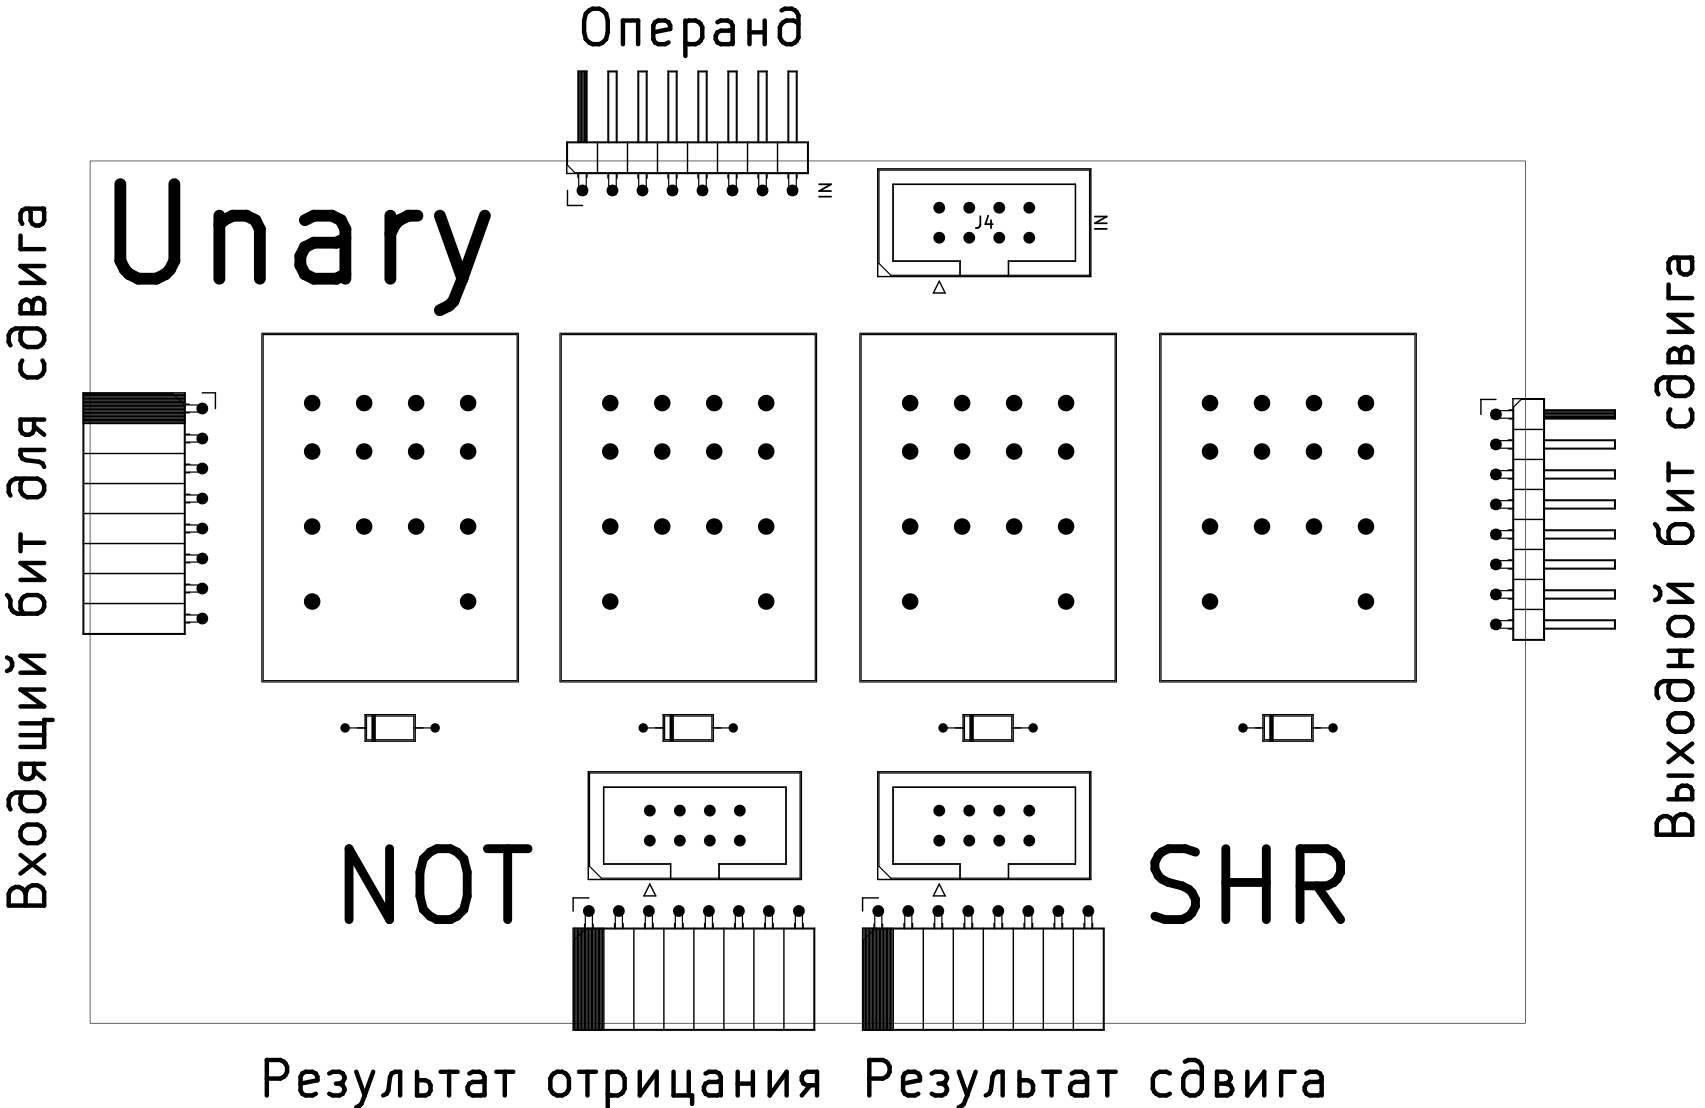
\includegraphics{boards/logic_unary.png}
\end{center}

Модуль для унарных операций выполняет действия над $4$-битным числом: сдвиг вправо и инверсия битов.

Может каскадироваться для сдвига $8$-битных чисел.

\subsection{Практикум}

На вход модуля унарных операций подключается модуль с тумблерами.
Выходы подключаются к шинам регистра.


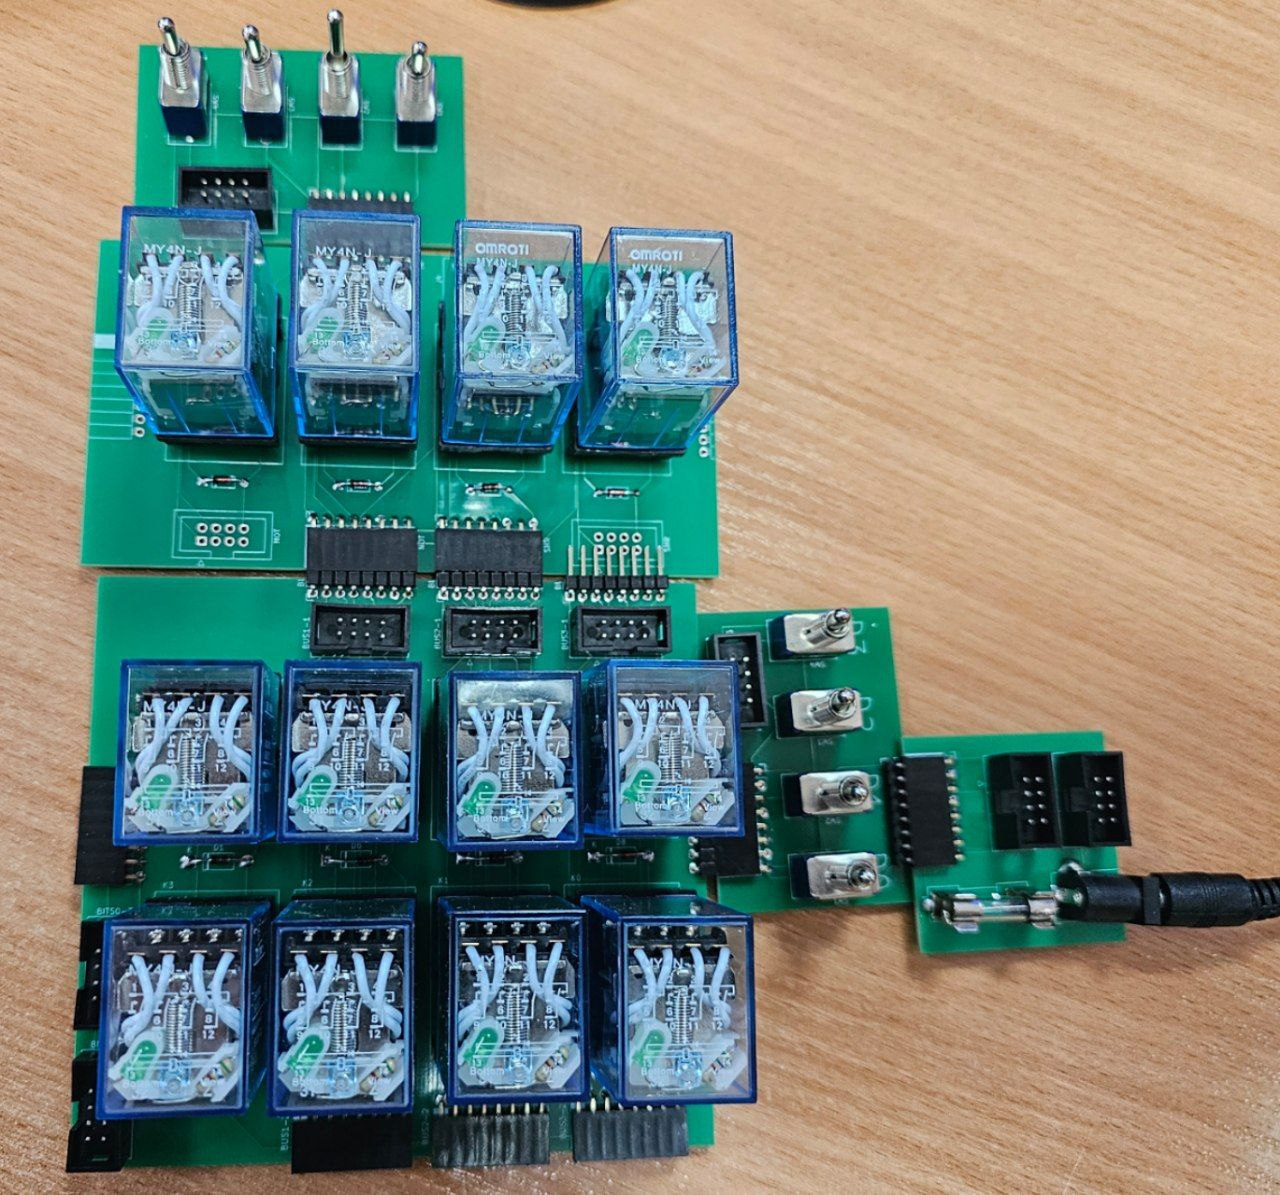
\includegraphics[width=0.5\columnwidth]{photo/unary.jpg}

\begin{enumerate}
    \item Отключить все управляющие сигналы.
    \item Набрать на тумблерах со входными данными значение $1100$.
    \item Подключить выходной регистр к шине $1$. Убедиться, что в него записалось значение $0011$ (инверсия).
    \item Отключить регистр от шины, сбросить его значение.
    \item Подключить выходной регистр к шине $2$. Убедиться, что в него записалось значение $0110$ (сдвиг вправо).
\end{enumerate}

\subsection{Задачи}

\begin{enumerate}
    \item Собрать устройство, позволяющее сдвигать содержимое регистра и записывать результат обратно.
          Занести в регистр значение $1000$ и сдвигать его до тех пор, пока не получится $0001$.
          Вторую часть можно выполнять на скорость.
\end{enumerate}


\section{Логическое И}

Реле представляет собой управляемый выключатель или переключатель.
Если на один контакт $A$ выключателя подать сигнал, то на другом $C$ он появится
только если на обмотке реле $B$ есть напряжение (логическая единица).

\begin{center}
\includegraphics{schemes/and.png}
\end{center}

Получается, что на выходе выключателя сигнал будет только тогда, когда
реле включено и на входе выключателя тоже не ноль. Это означает, что такая
схема реализует операцию логическое <<И>>: $C = A \land B$.



\section{Логическое ИЛИ}


Схему для выполнения логического <<ИЛИ>> можно получить, если соединить два выхода
(две цепи). Тогда напряжение на объединённом выходе появится в любом
из вариантов, если на первом выходе единица или на втором: $C = A \lor B$.

\begin{center}
\includegraphics{schemes/or1.png}
\end{center}

Но у этого способа есть один недостаток. Если на входе $A$ окажется единица,
то так как все входы и выходы соединены в одну цепь, поданное через $A$ напряжение
будет влиять и на вход $B$. И когда $B$ используется ещё где-то,
всё заработает неправильно, какое-то реле включится.
Такой вот паразитный сигнал --- $A$ влияет на выходы, зависящие от $B$.

Поэтому иногда стоит использовать схему с реле для логического <<ИЛИ>>:

\begin{center}
\includegraphics{schemes/or2.png}
\end{center}


\section{Исключающее ИЛИ}

Схема для вычисления <<исключающего или>> несколько сложнее.
Результат операции должен равняться единице только тогда,
когда операнды не равны. То есть если на одном из входов уже
было напряжение, а потом оно появляется и на другом входе,
выход из состояния единицы должен переключиться в ноль.

Такую логику проще всего реализовать с помощью двух переключающих контактов:

\begin{center}
\includegraphics{schemes/xor.png}
\end{center}

Благодаря перекрёстному соединению переключателей проводниками,
сигнал на выходе $C$ появляется только тогда, когда переключатели на реле
находятся в противоположных положениях.

\section{Бинарные логические операции}

\begin{center}
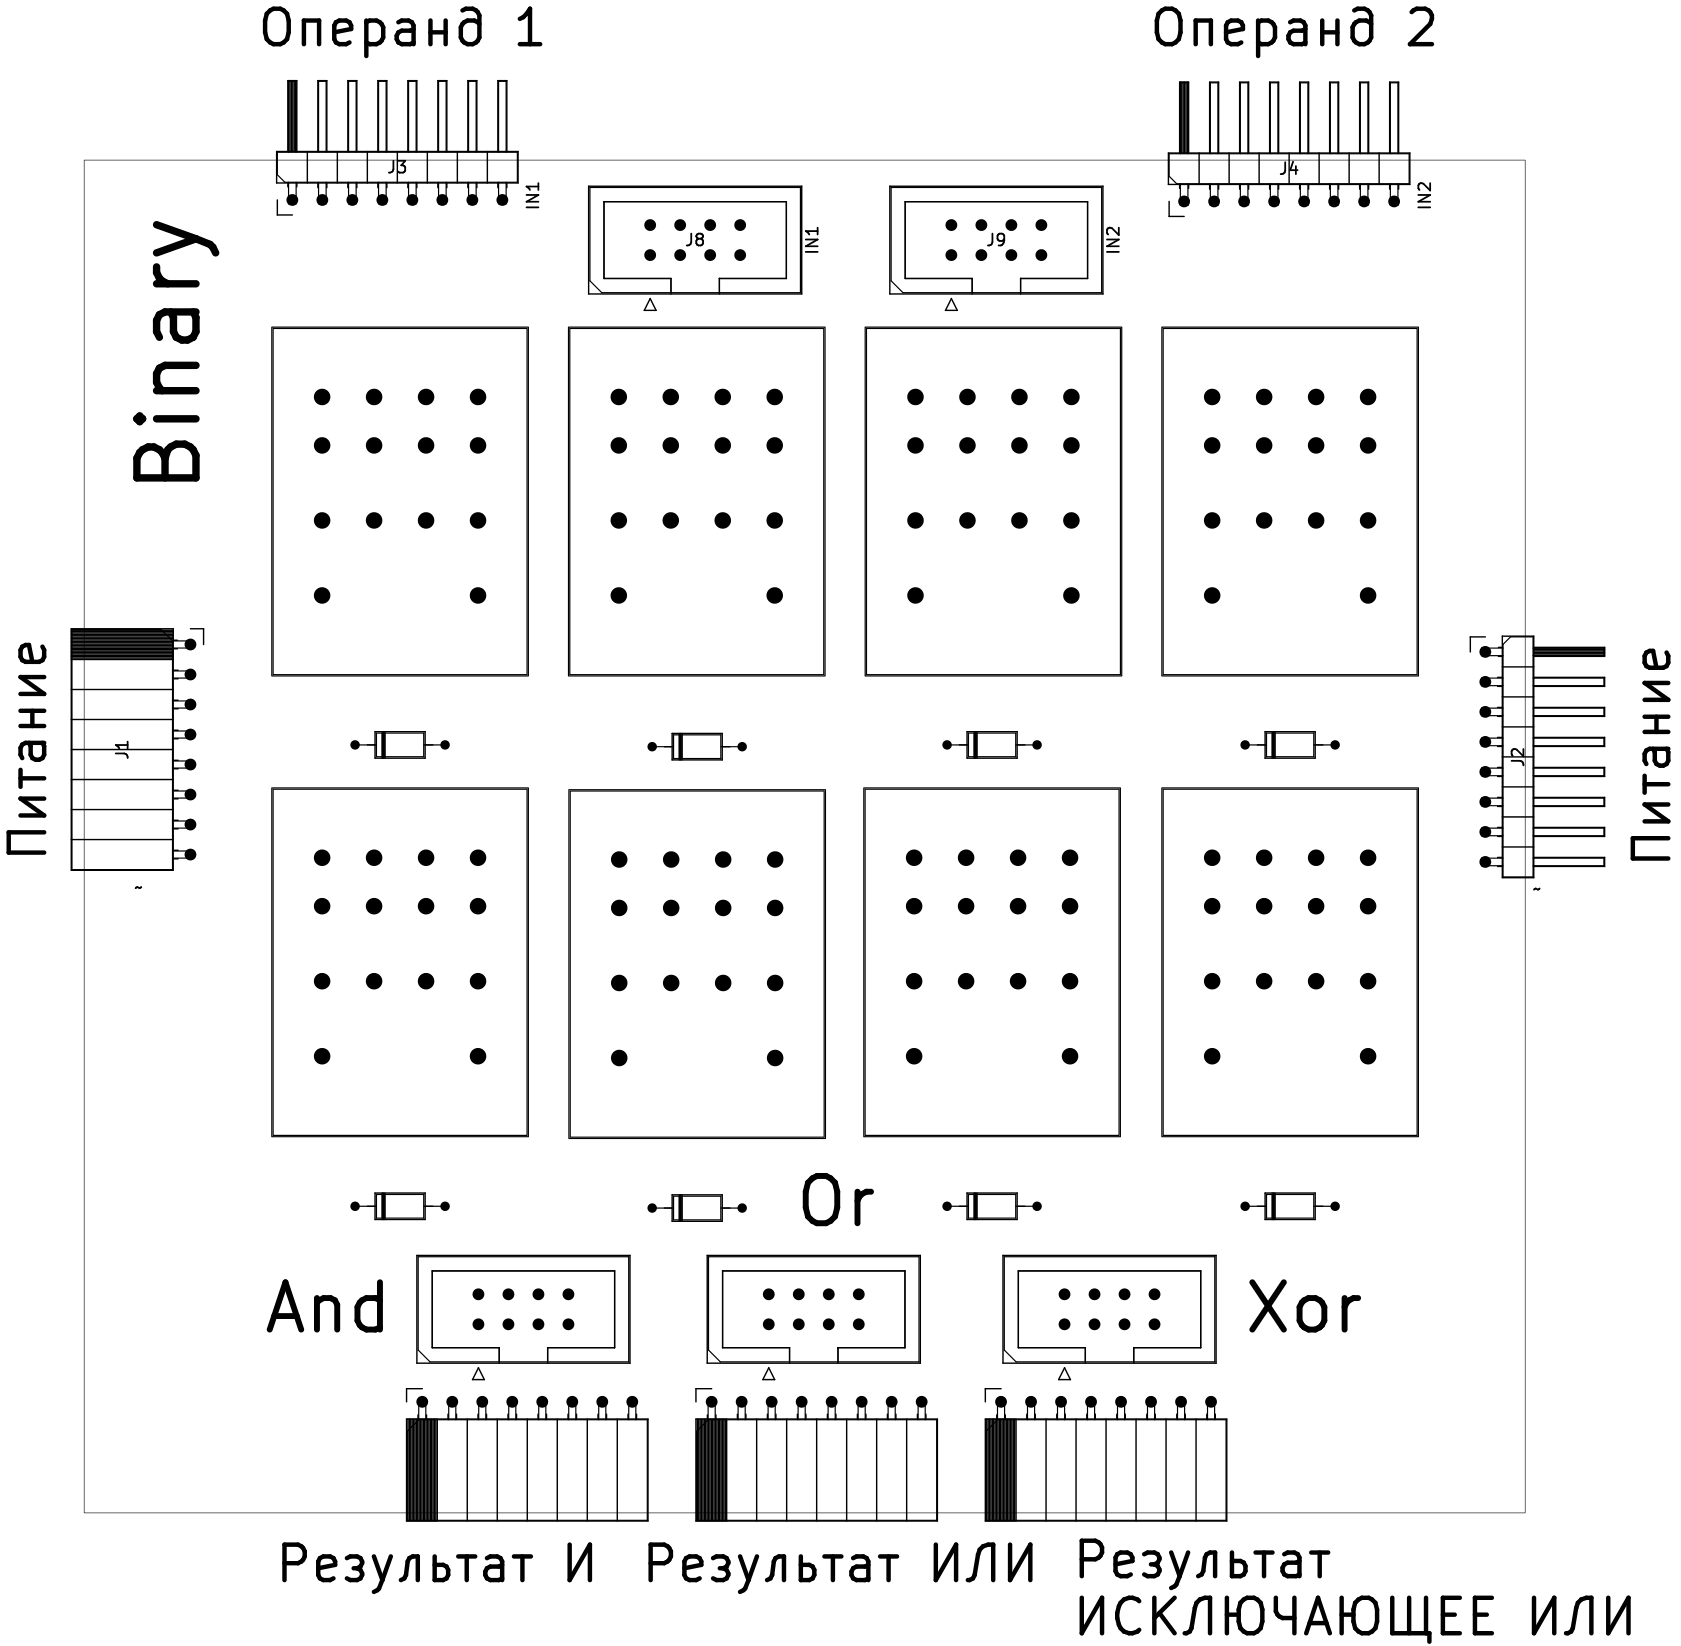
\includegraphics{boards/logic_binary.png}
\end{center}

Модуль логических операций поддерживает вычисление AND, OR и XOR.
У модуля есть два четырёхбитных входа и три выхода.
Каждый выход отвечает за одну операцию.

\subsection{Подготовка}

\begin{enumerate}
    \item Как могла бы выглядеть схема для выполнения операцию XOR?
\end{enumerate}

\subsection{Практикум}

Ко входам модуля подключаются два модуля с тумблерами, а к выходам --- регистр,
куда будет записываться результат.


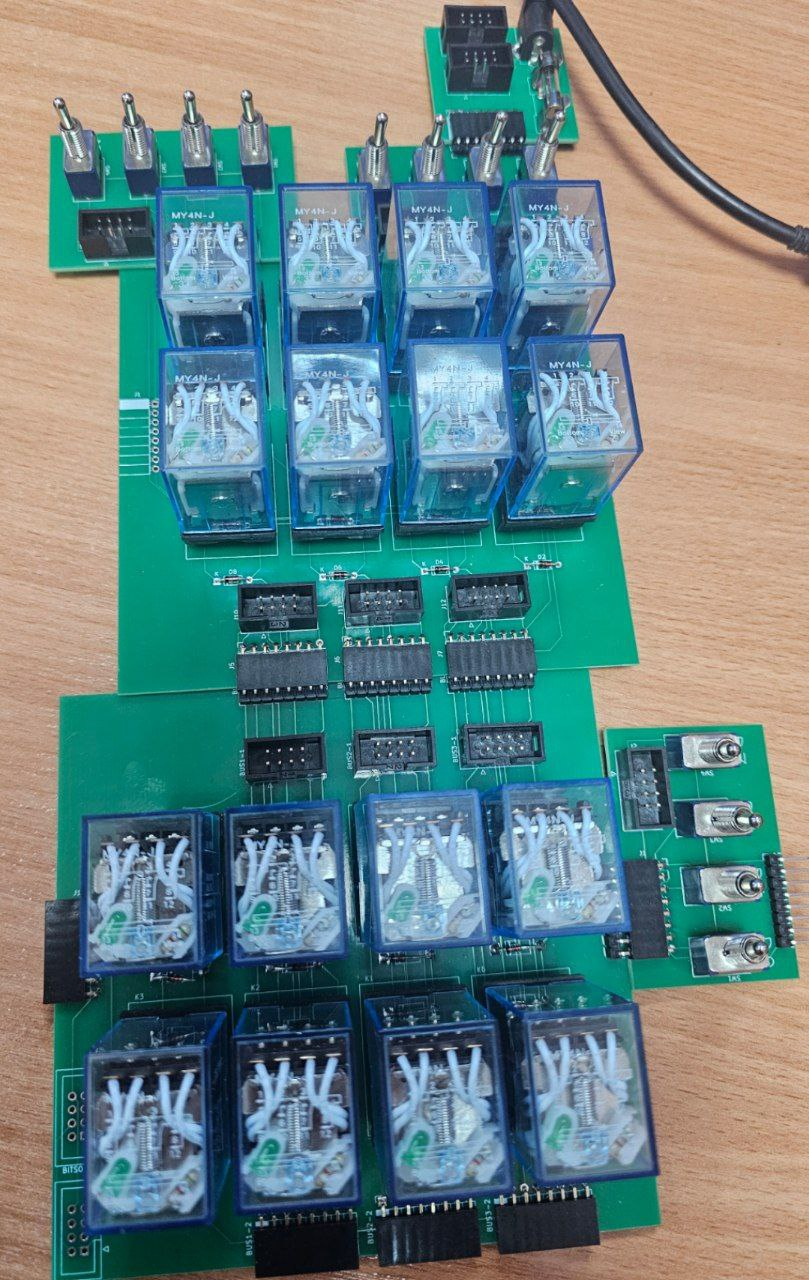
\includegraphics[width=0.5\columnwidth]{photo/logic.jpg}

\begin{enumerate}
    \item Отключить все управляющие сигналы.
    \item Набрать на тумблерах первого операнда значение $1100$.
    \item Набрать на тумблерах второго операнда значение $1010$.
    \item Подключить выходной регистр к шине $1$. Убедиться, что в него записалось значение $1000$ (AND).
    \item Отключить регистр от шины, сбросить его значение.
    \item Подключить выходной регистр к шине $2$. Убедиться, что в него записалось значение $1110$ (OR).
    \item Отключить регистр от шины, сбросить его значение.
    \item Подключить выходной регистр к шине $3$. Убедиться, что в него записалось значение $0110$ (XOR).
\end{enumerate}




\section{Шина и регистровый файл}

Несколько регистров можно соединить в регистровый файл.
У каждого из регистров есть сигналы выборки на одну из трёх шин.

Если два регистра подключены к одной шине одновременно,
то значения одного будут копироваться в другой. Если точнее,
включённые биты включают аналогичные в другом регистре, то есть
копирование возможно в обе стороны одновременно.

Нулевые биты при этом копироваться не могут. Для записи нулей
регистр необходимо сбросить.


\subsection{Практикум}


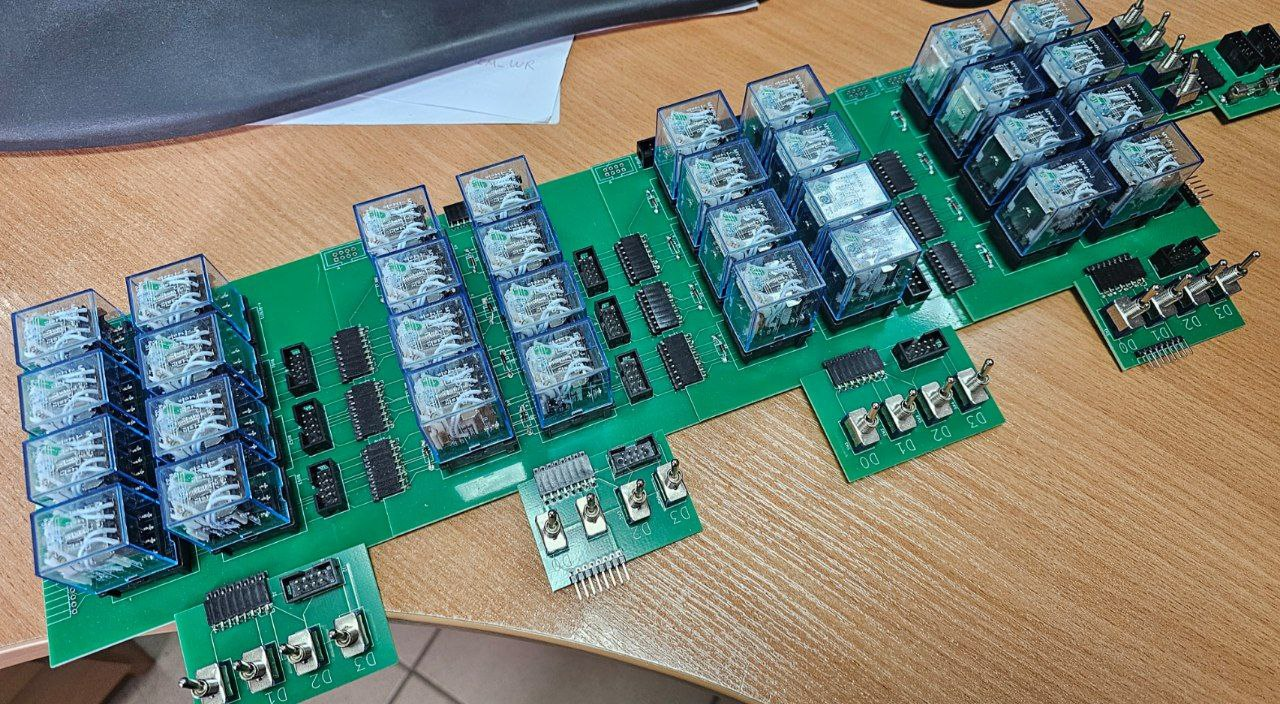
\includegraphics[width=\columnwidth]{photo/register_file.jpg}

Запись в регистры:

\begin{enumerate}
    \item Отключить все управляющие сигналы.
    \item Набрать значение на тумблерах, подключённых к шине данных $1$.
    \item Подключить с помощью тумблера регистр к шине $1$. Убедиться, что в него записалось набранное значение.
    \item Отключить регистр от шины.
    \item Подключить другой регистр к шине $1$. Убедиться, что в него записалось набранное значение.
\end{enumerate}

Копирование значения:

\begin{enumerate}
    \item Отключить все управляющие сигналы.
    \item Подключить регистр с ненулевыми битами к шине $2$.
    \item Подключить пустой регистр к шине $2$. убедиться, что он получил такое же значение, что и в первом регистре.
    \item Отключить все управляющие сигналы.
    \item Аналогично проверить шину $3$.
\end{enumerate}



\section{Арифметические операции}

\section{Сложение}

Чтобы складывать числа, сначала нужно научиться складывать отдельные биты.
Сумма двух битов может дать результат $0_2$, $1_2$ или $10_2$.
То есть при сложении получается уже двухбитовое число.

Схему сложения удобнее всего строить из однотипных компонентов, складывающих
фиксированное количество битов. На выходе такого компонента будет результат
сложения, а также бит переполнения (переноса). Для каскадирования
таких модулей нужно также иметь возможность подавать на вход перенос от
сумматоров младших битов.

Таким образом, сумматор получает на вход бит переноса и два числа, а на выходе
у него тоже бит переноса и число-сумма.


\section{Сумматор}

\begin{center}
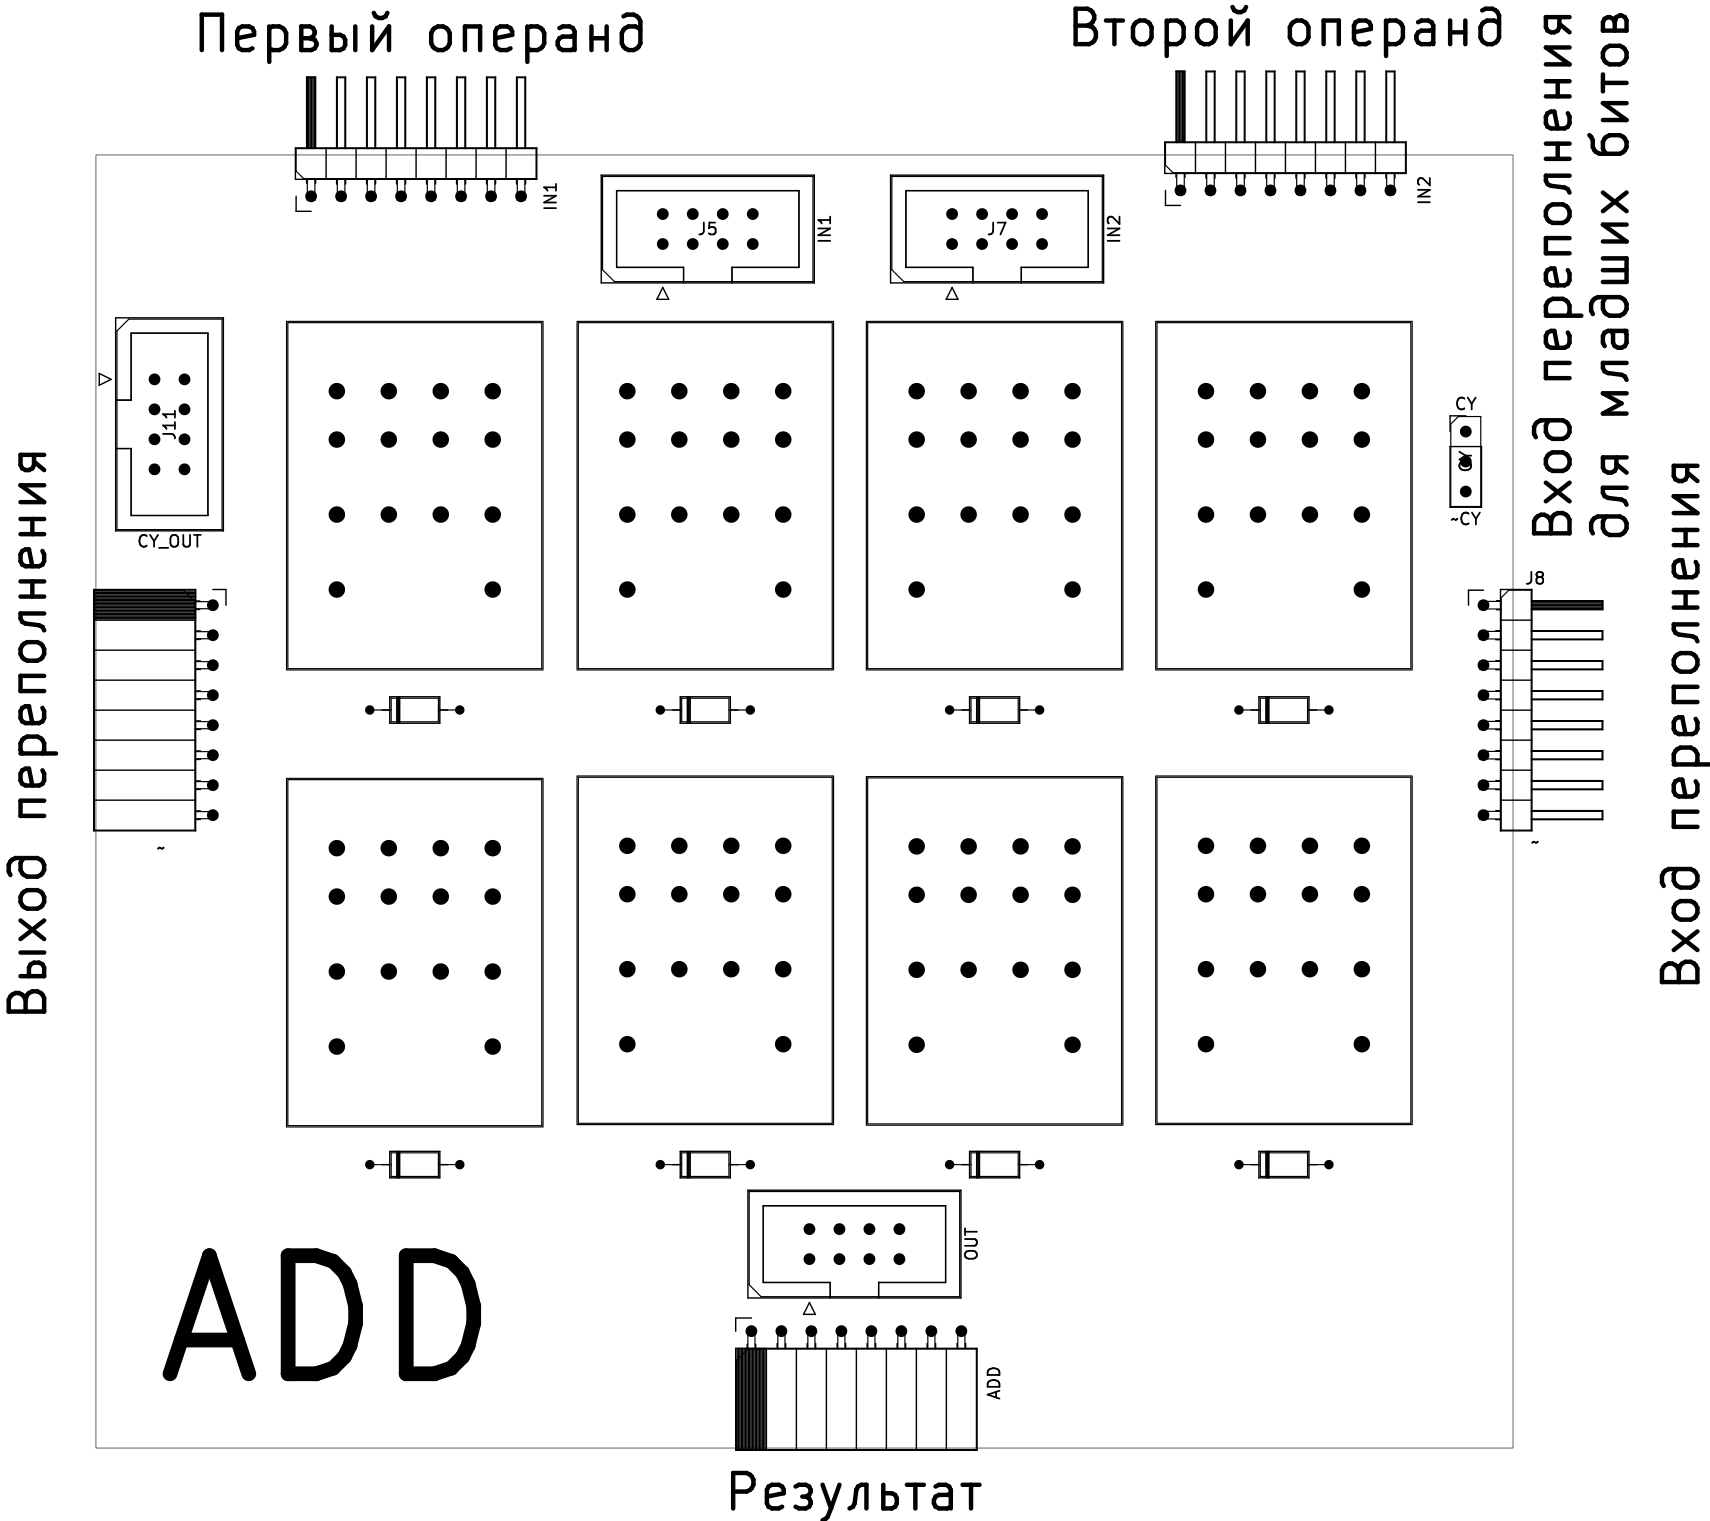
\includegraphics{boards/adder.png}
\end{center}

Сумматор складывает два четырёхбитных числа, один бит переноса и выдаёт четырёхбитное число и бит переноса.
У модуля есть два четырёхбитный вход и один выход.
Каждый выход отвечает за одну операцию.


\subsection{Подготовка}

\begin{enumerate}
    \item Придумайте, как можно было бы составить схему из реле, чтобы вычислять сумму однобитовых чисел.
    \item Как можно использовать предыдущую схему для вычисления суммы двухбитовых чисел?
\end{enumerate}

\subsection{Практикум}

Ко входам модуля подключаются два модуля с тумблерами, а к выходам --- регистр,
куда будет записываться результат.

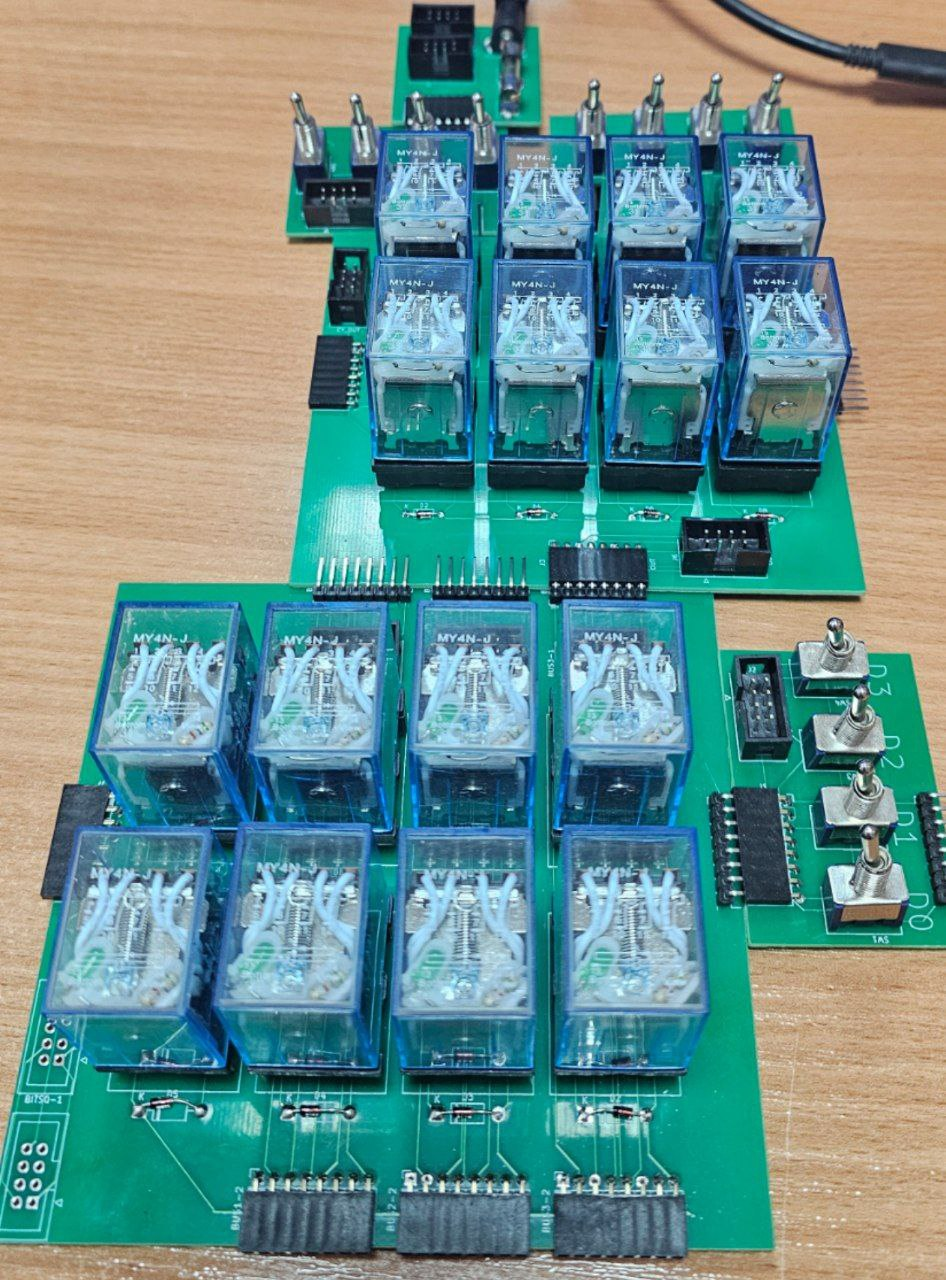
\includegraphics[width=0.5\columnwidth]{photo/adder.jpg}

\begin{enumerate}
    \item Отключить все управляющие сигналы.
    \item Установить перемычку для подачи сигнала на $~CY$.
    \item Набрать на тумблерах первого операнда значение $0011$ (число $3$).
    \item Набрать на тумблерах второго операнда значение $1010$ (число $10$).
    \item Подключить выходной регистр к шине $3$. Убедиться, что в него записалось значение $1101$ (число $13$).
    \item Отключить регистр от шины, сбросить его значение.
    \item Установить перемычку для подачи сигнала на $CY$.
    \item Подключить выходной регистр к шине $3$. Убедиться, что в него записалось значение $1110$ (число $14$).
\end{enumerate}


\subsection{Задачи}

\begin{enumerate}
    \item Собрать устройство для сложения значения из регистра с константой, набранной на тумблерах.
          Должна быть предусмотрена запись результата обратно в регистр.
          Дальше управлять сигналами таким образом, чтобы к регистру последовательно
          прибавлялась единица, пока он не достигнет значения $1111$.
\end{enumerate}



\section{Вычитание}

\subsection{Вычитание через сложение с дополнительным обратным кодом}

Чтобы вычесть из одного числа другое, можно вычитаемое представить в дополнительном обратном
коде, а затем сложить это число с уменьшаемым.

Число в дополнительном обратном коде получается, если сначала инвертировать биты исходного
числа, а затем прибавить к нему единицу.

Например, для числа $3=0011$ инверсия будет выглядеть, как $1100$, а дополнительный обратный код, как $1101$.

\subsubsection{Практикум}

Собрать схему для сложения.

\begin{enumerate}
    \item Отключить все управляющие сигналы.
    \item Установить перемычку для подачи сигнала на $~CY$.
    \item Набрать на тумблерах первого операнда значение $1010$ (число $10$).
    \item Набрать на тумблерах второго операнда значение $1101$ (число $-3$).
    \item Подключить выходной регистр к шине $3$. Убедиться, что в него записалось значение $0111$ (число $7$).
\end{enumerate}

\subsubsection{Задачи}
\begin{enumerate}
    \item Выполните деление в столбик числа $14$ на $3$ с помощью последовательности вычитаний.
          Записывайте промежуточные результаты на бумаге.
    \item Сделайте то же самое, только сохраняйте все промежуточные результаты в разных
          регистрах регистрового файла.
\end{enumerate}

\subsection{Вычитание с помощью сумматора и инвертора}

Вычитание можно делать с помощью сумматора. Чтобы на входе из операнда получался дополнительный
обратный код, сначала нужно преобразовать его с помощью инвертора, а затем прибавить $1$,
включив вход переноса в сумматоре.

\subsubsection{Практикум}

Собрать схему для сложения, а затем добавить между тумблерами со вторым операндом
инвертор (выход NOT блока унарной логики):

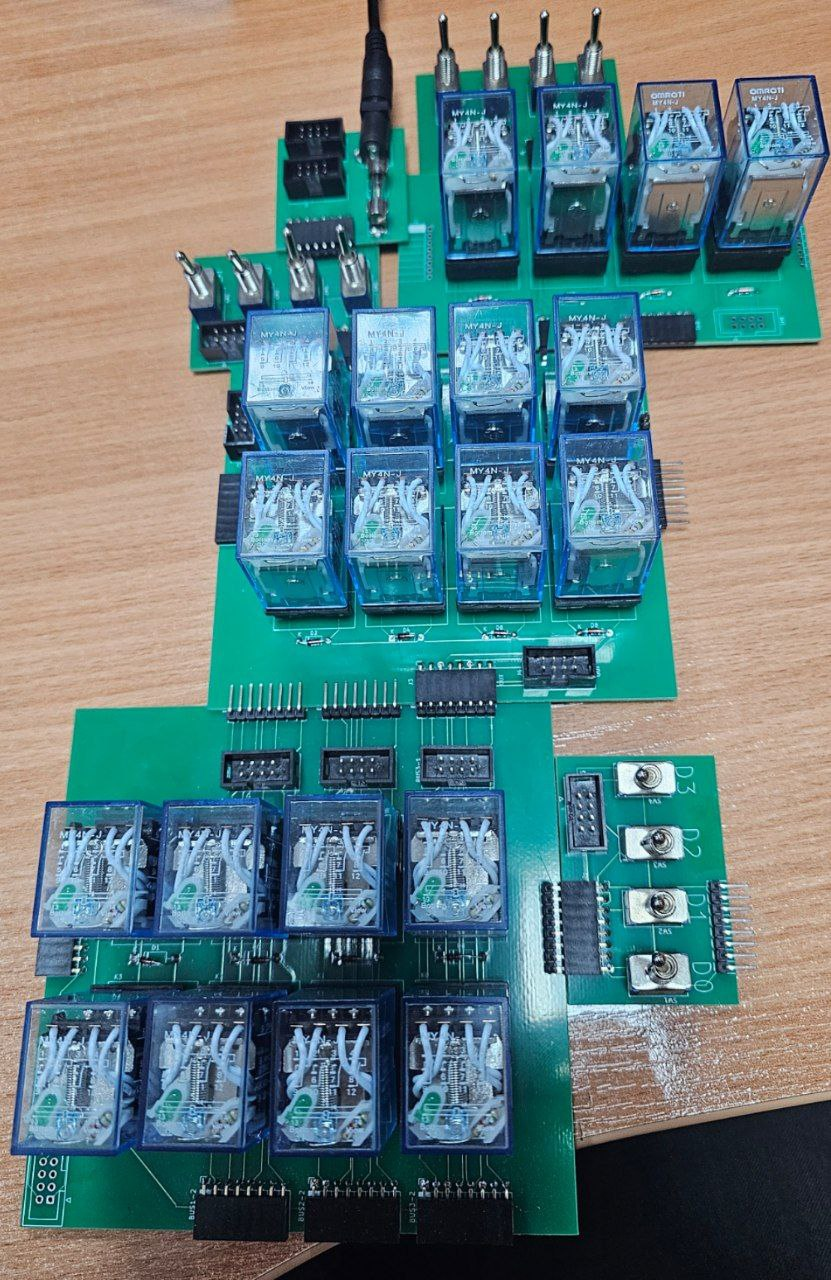
\includegraphics[width=0.5\columnwidth]{photo/subtractor.jpg}

\begin{enumerate}
    \item Отключить все управляющие сигналы.
    \item Установить перемычку для подачи сигнала на $CY$.
    \item Набрать на тумблерах первого операнда значение $1010$ (число $10$).
    \item Набрать на тумблерах второго операнда значение $0011$ (число $3$).
    \item Подключить выходной регистр к шине $3$. Убедиться, что в него записалось значение $0111$ (число $7$).
\end{enumerate}
